\documentclass[../Carre_nights.tex]{subfiles}

\begin{document}

\section{n0825}
\textbf{\Large{The tale of the unending treasure}} \\

\begin{figure}[ht]
\centering
\includegraphics[height=\figsize]{illustrations/volume_7/T07, n0825 - Le trésor sans fond.jpg}
\end{figure}

\textit{\\
"...un bassin d’albâtre blanc, de cent pieds de circonférence, se voyait au milieu de cette salle, plein de pièces d’or et de tous les joyaux que peut rêver le cerveau le plus exalté."} \\
—T07, n0825 - Le trésor sans fond \\~\\
\textit{"...he saw a pond of white alabaster, one hundred feet in circumference, which was filled entirely with gold pieces."} \\
—V04, n0825 - The tale of the unending treasure

\newpage

\section{n0833}
\textbf{\Large{The adventures of the royal bastard [The tale of the ape youth]}} \\

\begin{figure}[ht]
\centering
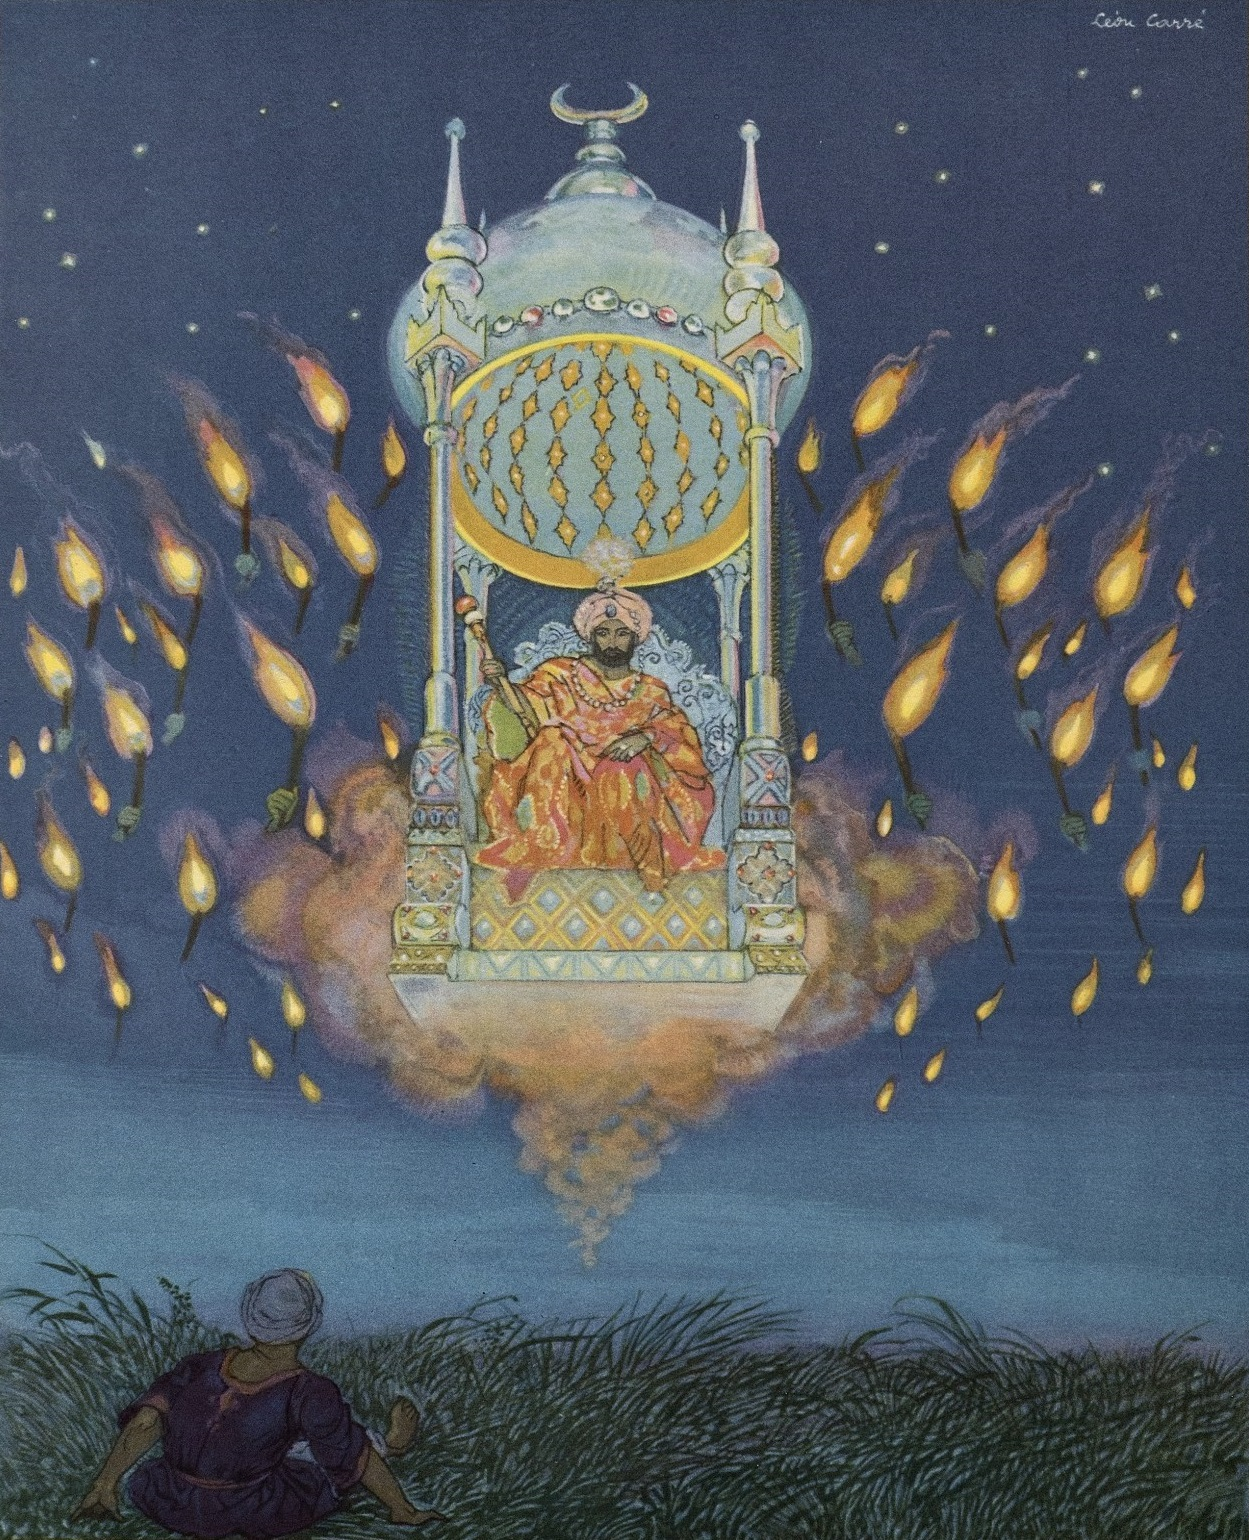
\includegraphics[height=\figsize]{illustrations/volume_7/T07, n0833 - Histoire compliquée de l’adultérin sympathique [Histoire du singe jouvenceau].jpg}
\end{figure}

\textit{\\
"...un nombre infini de flambeaux, portés par des mains sans propriétaires, passèrent de la sorte deux à deux devant moi. Et enfin je vis, entouré d’un grand nombre de lumières, un roi sur son trône, revêtu de splendeur."} \\
—T07, n0833 - Histoire compliquée de l’adultérin sympathique [Histoire du singe jouvenceau] \\~\\
\textit{"...I beheld a great number of torches, which seemed to be borne along in the distance; but the hands which carried them and the folk they lighted were invisible. Soon, where the torches were the thickest, I saw a King borne by on his throne."} \\
—V04, n0833 - The adventures of the royal bastard [The tale of the ape youth]

\newpage

\section{n0840}
\textbf{\Large{The adventures of the royal bastard [The second madman’s tale]}} \\

\begin{figure}[ht]
\centering
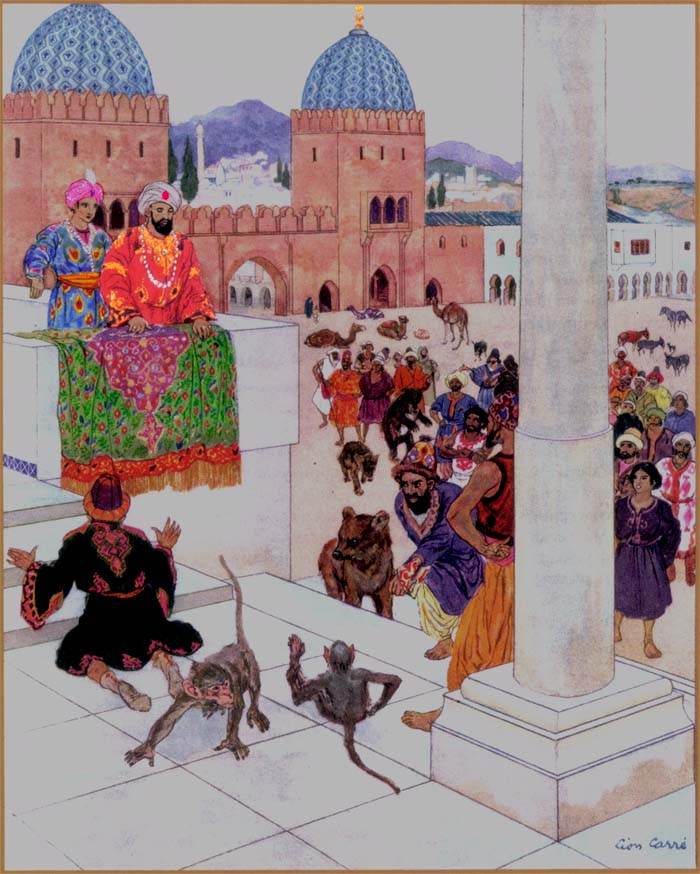
\includegraphics[height=\figsize]{illustrations/volume_7/T07, n0840 - Histoire compliquée de l’adultérin sympathique [Histoire du deuxième fou].jpg}
\end{figure}

\textit{\\
"...ils étaient tous là, les conducteurs de singes avec leurs animaux, les montreurs d’ours avec leurs plus beaux sujets, les bouffons avec leurs oripeaux, les charlatans avec leurs hauts bonnets de feutre, et les instrumentistes avec leurs bruyants instruments dont s’exhalait un immense hourvari."} \\
—T07, n0840 - Histoire compliquée de l’adultérin sympathique [Histoire du deuxième fou] \\~\\
\textit{"Ape leaders led their apes, bear masters showed their bears, buffoons twirled their tinsel, quacks cocked their high felt bonnets, singers of lewd songs sang their lewd songs, and players upon instruments played upon their instruments, altogether and all out of tune."} \\
—V04, n0840 - The adventures of the royal bastard [The second madman’s tale]

\newpage

\section{n0842}
\textbf{\Large{The adventures of the royal bastard [The second madman’s tale]}} \\

\begin{figure}[ht]
\centering
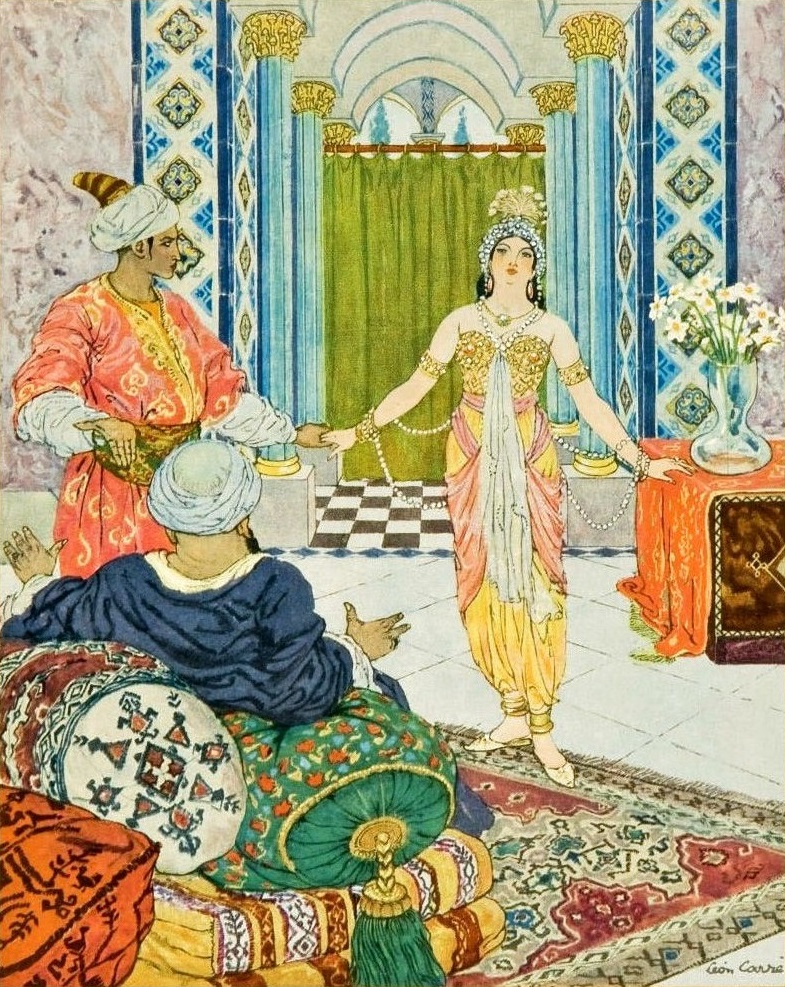
\includegraphics[height=\figsize]{illustrations/volume_7/T07, n0842 - Histoire compliquée de l’adultérin sympathique [Histoire du deuxième fou].jpg}
\end{figure}

\textit{\\
"...« Ô fille de l’oncle, je t’amène ton époux, cet excellent gaillard que je nomme à l’instant mon second chambellan, et qui sera désormais mon commensal et mon compagnon de coupe."} \\
—T07, n0842 - Histoire compliquée de l’adultérin sympathique [Histoire du deuxième fou] \\~\\
\textit{"'Child of my uncle,' he said, 'I bring you your husband, whom I have appointed my second chamberlain, my friend and cup-companion..."} \\
—V04, n0842 - The adventures of the royal bastard [The second madman’s tale]

\newpage

\section{n0849}
\textbf{\Large{The perfidy of wives [The greengrocer’s tale]}} \\

\begin{figure}[ht]
\centering
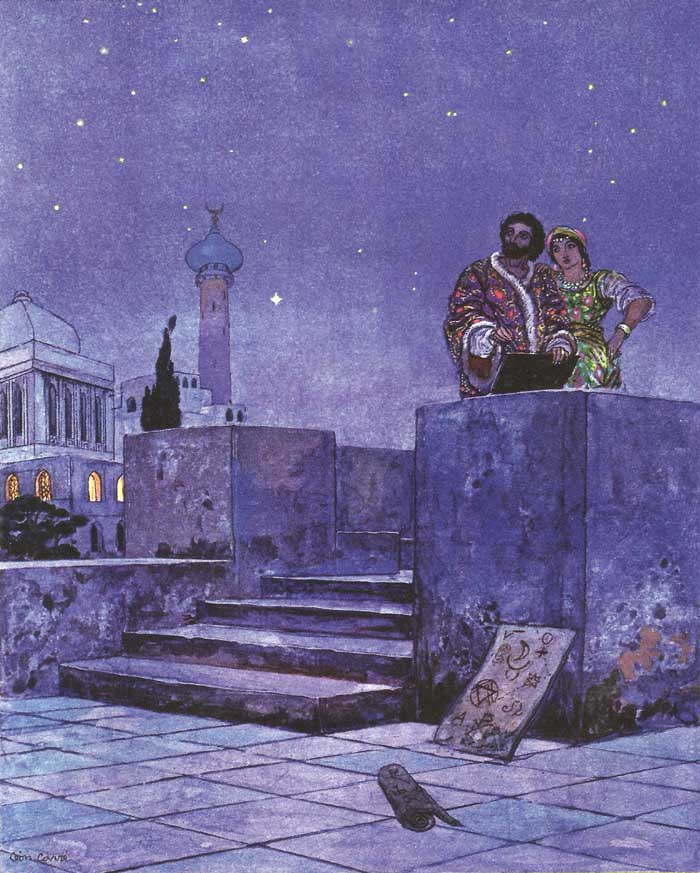
\includegraphics[height=\figsize]{illustrations/volume_7/T07, n0849 - La malice des épouses [Histoire racontée par le marchand de légumes].jpg}
\end{figure}

\textit{\\
"...il y avait un homme qui était astronome, de son métier, et qui savait lire sur les visages et deviner les pensées par la physionomie. Et cet astronome avait une épouse qui était d’une insigne beauté et d’un charme singulier."} \\
—T07, n0849 - La malice des épouses [Histoire racontée par le marchand de légumes] \\~\\
\textit{"...there was once a great astronomer who was also deeply learned in the reading of faces and the divining of hidden thoughts. He had a very beautiful wife..."} \\
—V04, n0849 - The perfidy of wives [The greengrocer’s tale]

\newpage

\section{n0851}
\textbf{\Large{The tale of Ali Baba and the forty thieves}} \\

\begin{figure}[ht]
\centering
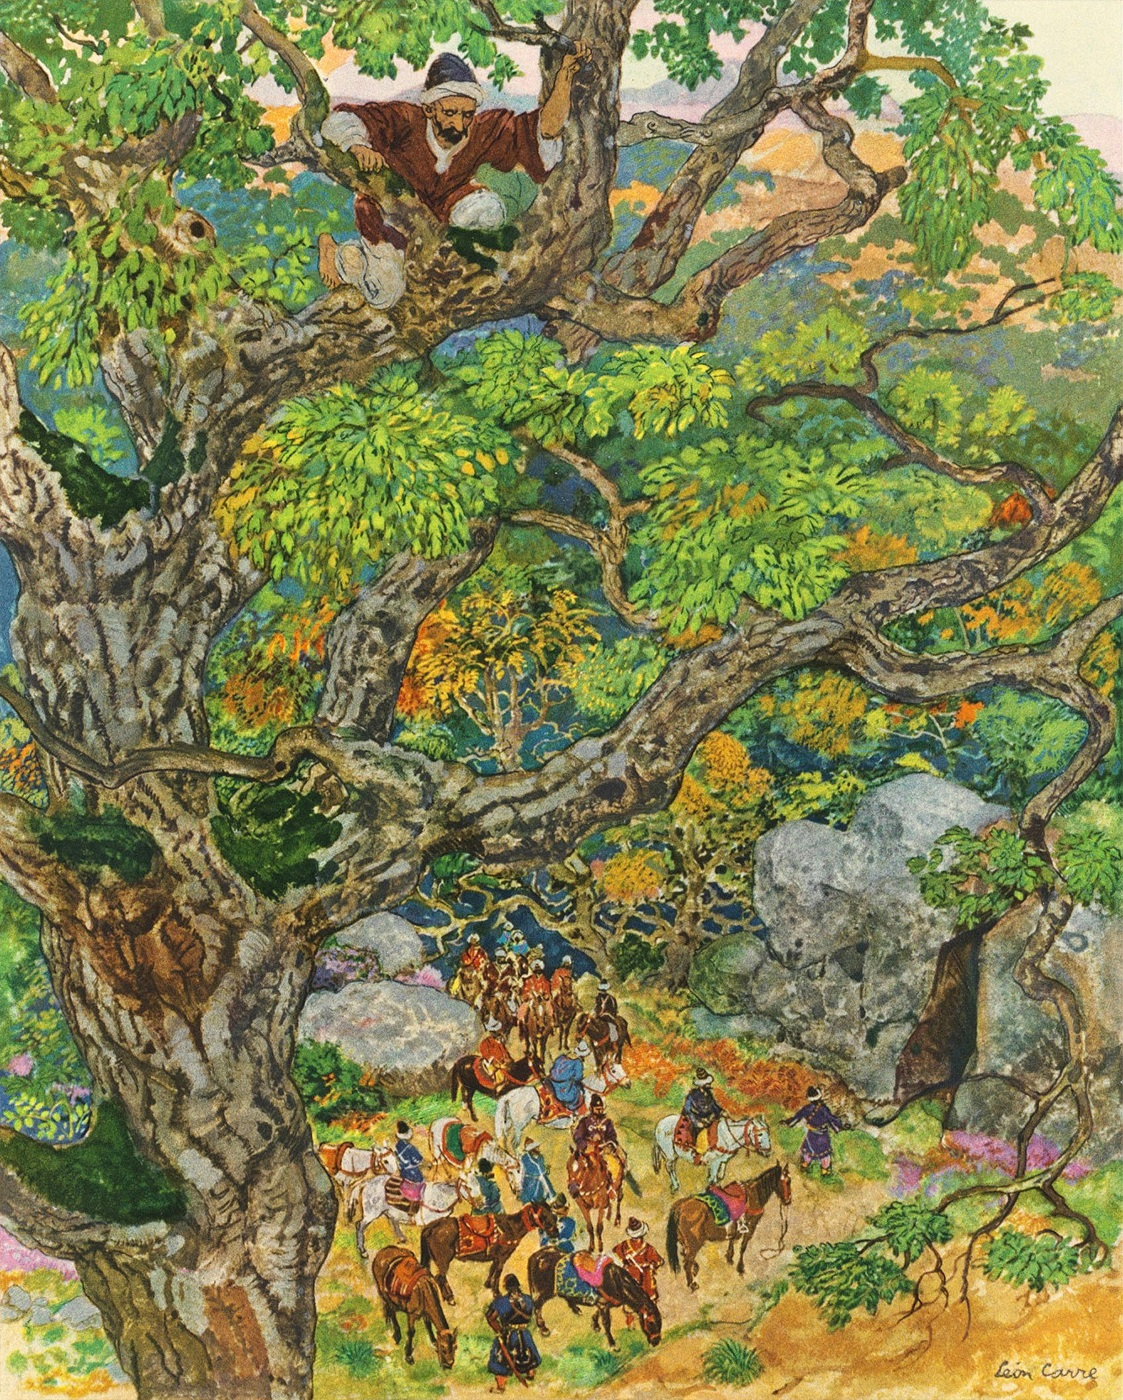
\includegraphics[height=\figsize]{illustrations/volume_7/T07, n0851 - Histoire d'Ali Baba et des quarante voleurs.jpg}
\end{figure}

\textit{\\
"...il put, ainsi posté et caché entre les branches, examiner quelle pouvait bien être l’affaire. Or, il fit bien ! Car il était à peine là, qu’il aperçut une troupe de cavaliers armés terriblement qui, d’un bon train, s’avançaient du côté où il se trouvait."} \\
—T07, n0851 - Histoire d'Ali Baba et des quarante voleurs \\~\\
\textit{"He had done well to hide himself, for soon a troop of armed riders came towards the tree..."} \\
—V04, n0851 - The tale of Ali Baba and the forty thieves

\newpage

\section{n0855}
\textbf{\Large{The tale of Ali Baba and the forty thieves}} \\

\begin{figure}[ht]
\centering
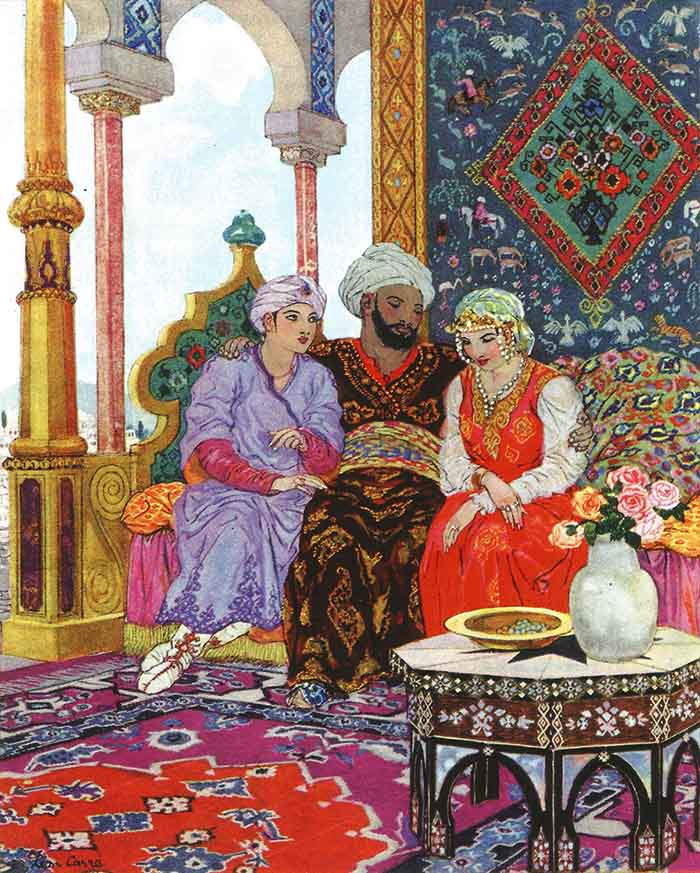
\includegraphics[height=\figsize]{illustrations/volume_7/T07, n0855 - Histoire d'Ali Baba et des quarante voleurs.jpg}
\end{figure}

\textit{\\
"Si donc, dans ce malheur sans remède qui t’atteint, quelque chose est encore capable de te consoler, je t’offre de joindre les biens qu’Allah m’a envoyés à ceux qui t’appartiennent, et à te faire entrer désormais dans ma maison en qualité de seconde épouse."} \\
—T07, n0855 - Histoire d'Ali Baba et des quarante voleurs \\~\\
\textit{"...if it would be any consolation to you in your great grief to accept your share of what I have and to remain in this house as my second wife, you are very welcome."} \\
—V04, n0855 - The tale of Ali Baba and the forty thieves

\newpage

\section{n0859}
\textbf{\Large{The tale of Ali Baba and the forty thieves}} \\

\begin{figure}[ht]
\centering
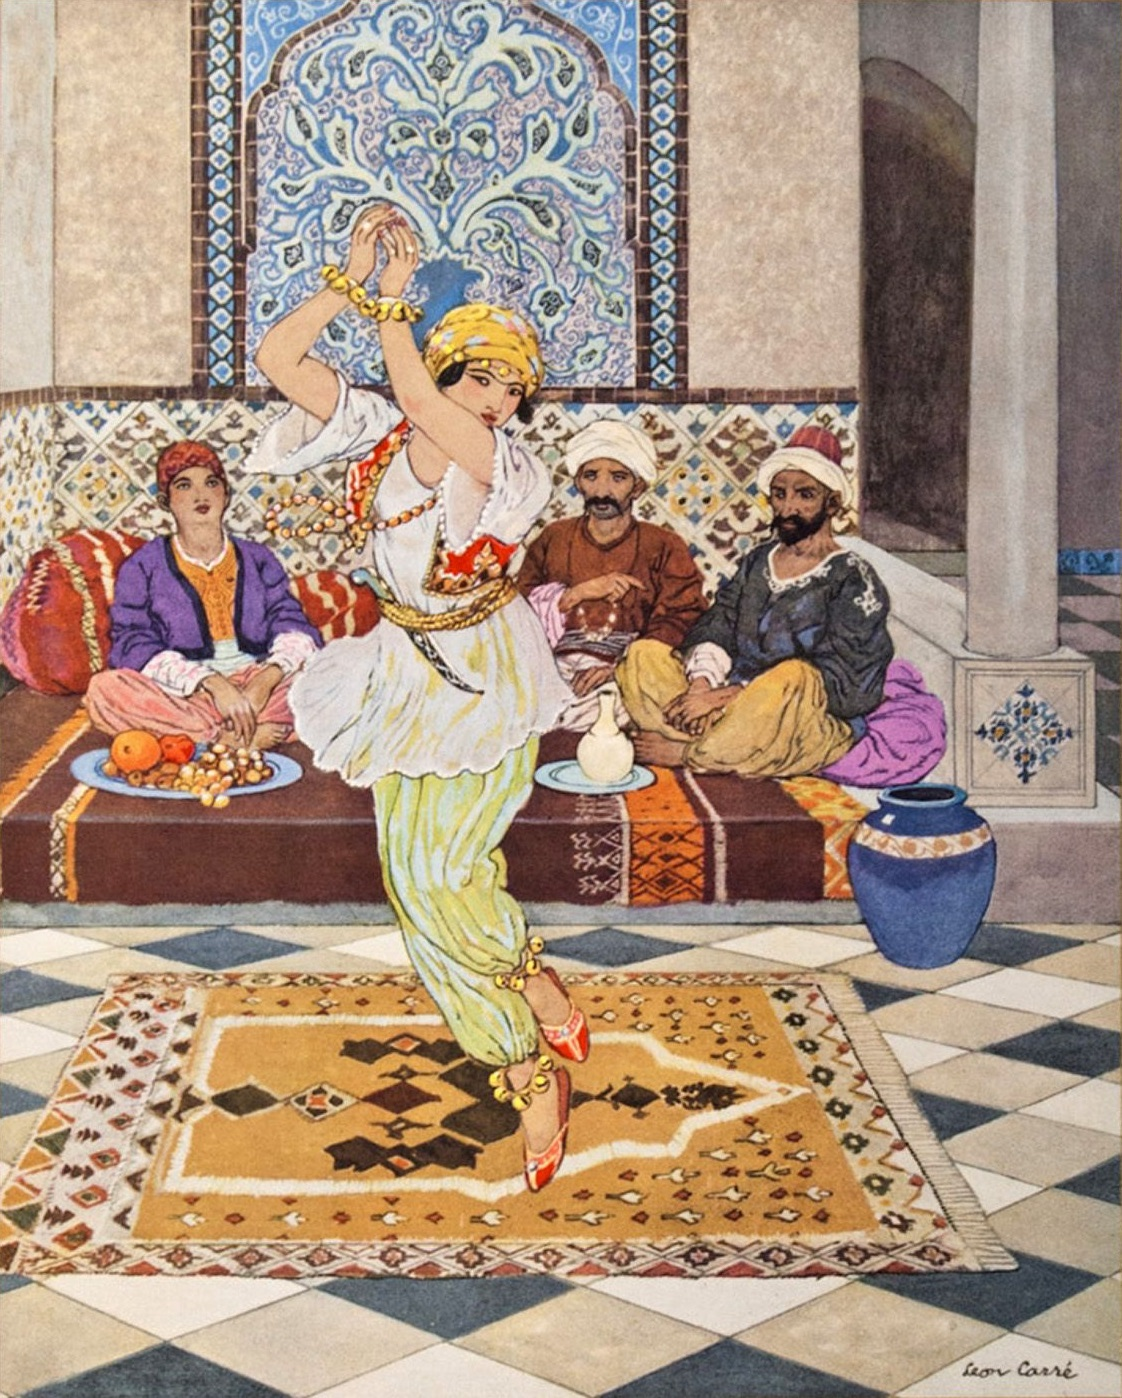
\includegraphics[height=\figsize]{illustrations/volume_7/T07, n0859 - Histoire d'Ali Baba et des quarante voleurs.jpg}
\end{figure}

\textit{\\
"Et elle dansa tous les pas, inlassable, et esquissa toutes les figures, comme jamais ne l’avait fait, dans les palais des rois, une danseuse de profession. Et elle dansa comme seul peut-être, devant Saül noir de tristesse, avait dansé le berger David."} \\
—T07, n0859 - Histoire d'Ali Baba et des quarante voleurs \\~\\
\textit{"She danced tirelessly and with all perfection, as the shepherd David danced before the black sadness of Saul."} \\
—V04, n0859 - The tale of Ali Baba and the forty thieves

\newpage

\section{n0860}
\textbf{\Large{The meetings of Al-Rashid}} \\

\begin{figure}[ht]
\centering
\includegraphics[height=\figsize]{illustrations/volume_7/T07, n0860 - Les rencontres d’Al-Rachid.jpg}
\end{figure}

\textit{\\
"...ils virent s’avancer sur le pont un magnifique cortège, comme n’en peuvent d’ordinaire déployer que les rois et les sultans."} \\
—T07, n0860 - Les rencontres d’Al-Rachid \\~\\
\textit{"...they saw a magnificent procession coming towards them, such as might be supposed only to attend upon kings."} \\
—V04, n0860 - The meetings of Al-Rashid

\newpage

\section{n0863}
\textbf{\Large{The meetings of Al-Rashid [The youth]}} \\

\begin{figure}[ht]
\centering
\includegraphics[height=\figsize]{illustrations/volume_7/T07, n0863 - Les rencontres d’Al-Rachid [Histoire du jeune homme].jpg}
\end{figure}

\textit{\\
"...elle laissa derrière elle le premier cimetière, dont les tombes étaient excessivement anciennes, et se hâta vers celui où l’on continuait à enterrer journellement."} \\
—T07, n0863 - Les rencontres d’Al-Rachid [Histoire du jeune homme] \\~\\
\textit{"The first cemetery, whose tombs are very old, she left behind her, and hastened to the one used for daily burial."} \\
—V04, n0863 - The meetings of Al-Rashid [The youth]

\newpage

\section{n0873}
\textbf{\Large{The meetings of Al-Rashid [The generous sheikh]}} \\

\begin{figure}[ht]
\centering
\includegraphics[height=\figsize]{illustrations/volume_7/T07, n0873 - Les rencontres d’Al-Rachid [Histoire du cheikh].jpg}
\end{figure}

\textit{\\
"...le portier leur fit traverser une forêt d’orangers et de citronniers chargés de fruits et dont les racines se rafraîchissaient à une eau vive qui coulait perpétuellement dans une rigole prenant sa source à la rivière."} \\
—T07, n0873 - Les rencontres d’Al-Rachid [Histoire du cheikh] \\~\\
\textit{"The porter led them through a forest of orange and lemon trees, whose roots were refreshed by living water seeping through little channels from the river..."} \\
—V04, n0873 - The meetings of Al-Rashid [The generous sheikh]

\newpage

\section{n0875}
\textbf{\Large{The meetings of Al-Rashid [The blind man]}} \\

\begin{figure}[ht]
\centering
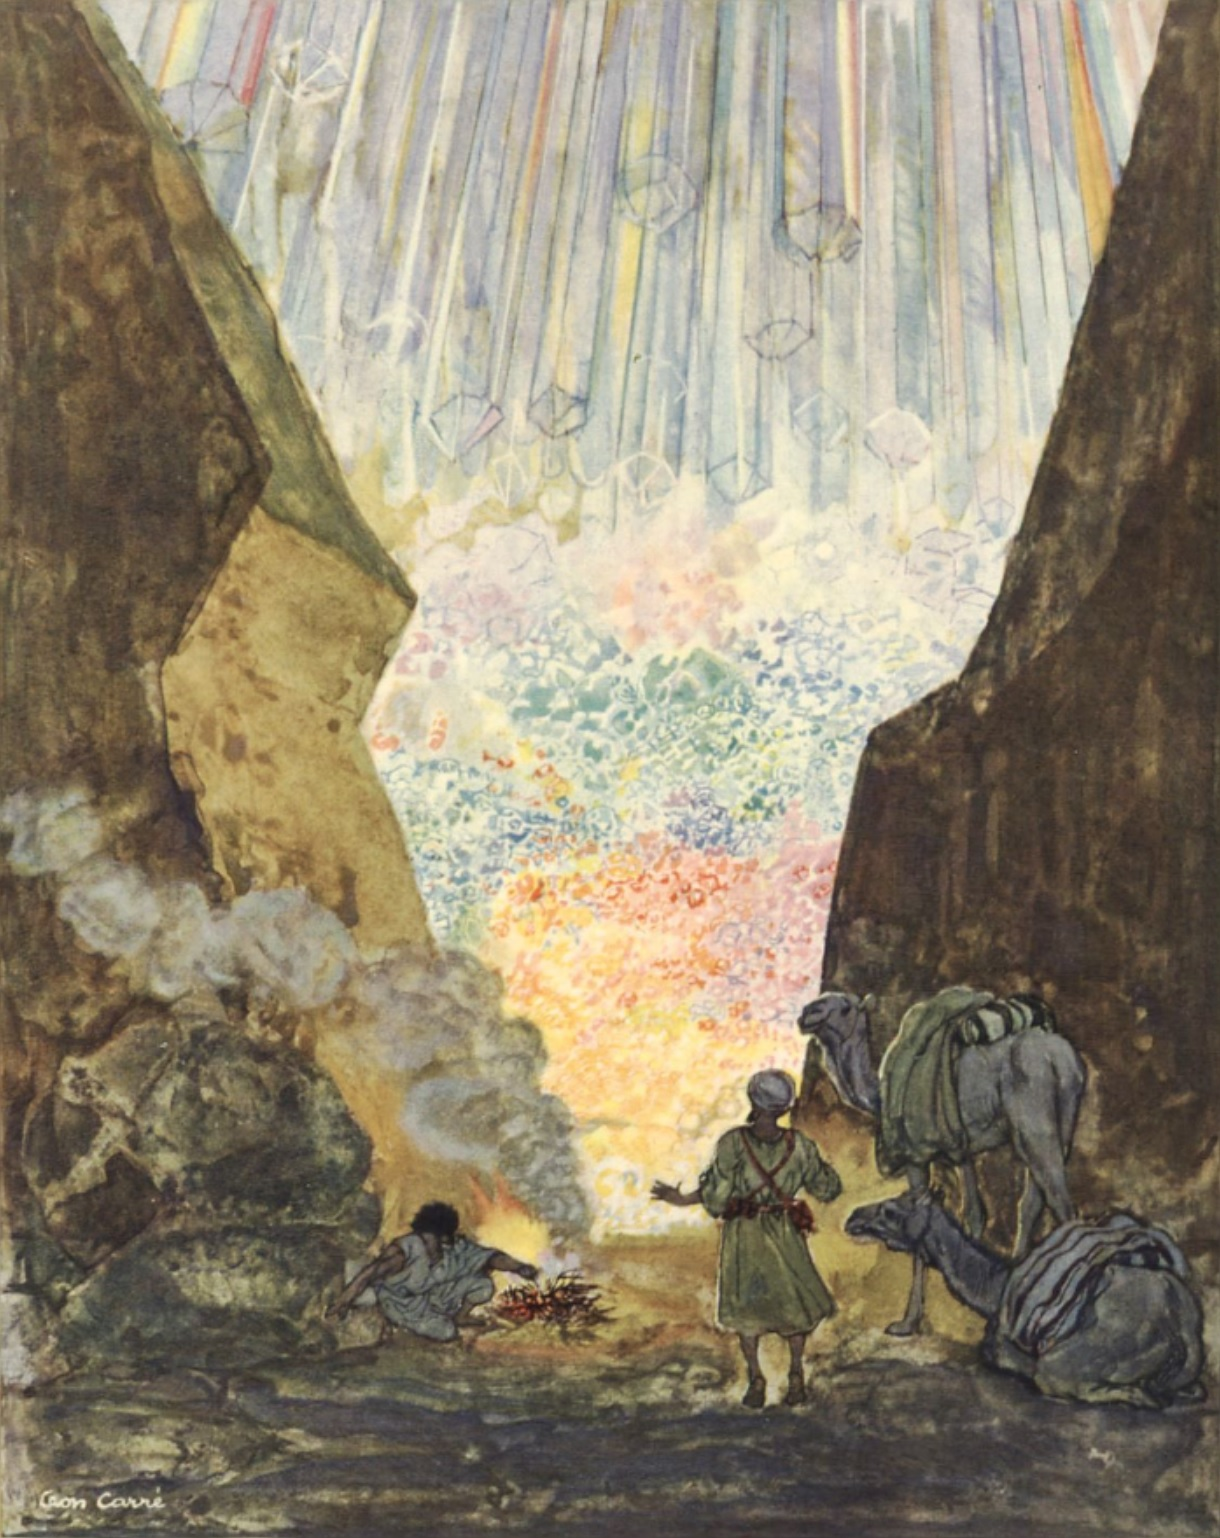
\includegraphics[height=\figsize]{illustrations/volume_7/T07, n0875 - Les rencontres d'Al-Rachid [Histoire de l'aveugle].jpg}
\end{figure}

\textit{\\
"...là-dedans, des monceaux s’étendaient d’or monnayé et de pierreries, comme ces tas de sel qu’on voit sur le bord de la mer."} \\
—T07, n0875 - Les rencontres d'Al-Rachid [Histoire de l'aveugle] \\~\\
\textit{"Within were hummocks of coined gold and bright jewels, massed as one sees salt upon the sea shore."} \\
—V04, n0875 - The meetings of Al-Rashid [The blind man]

\newpage

\section{n0881}
\textbf{\Large{The tale of princess Zulaikah}} \\

\begin{figure}[ht]
\centering
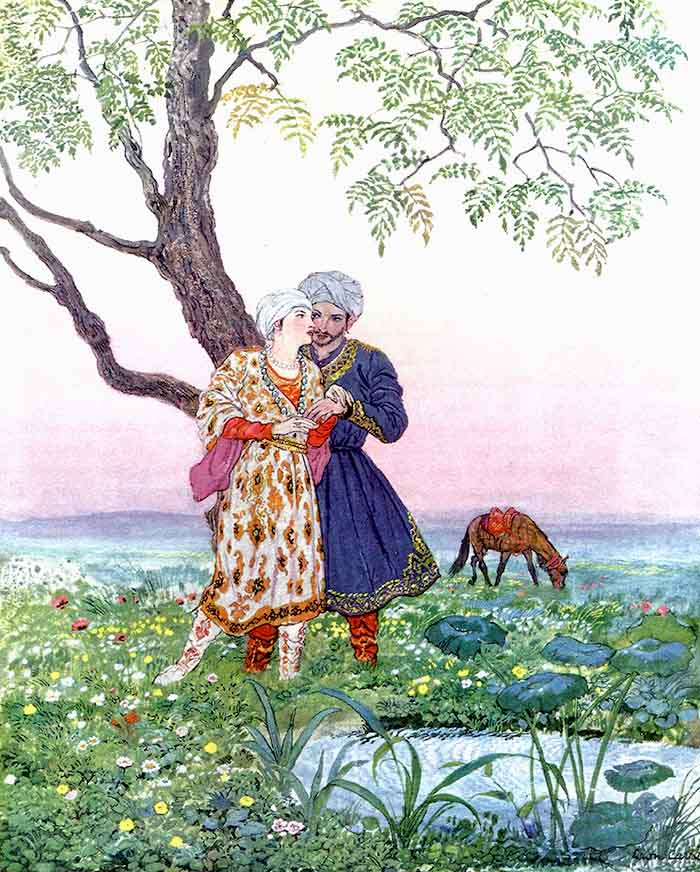
\includegraphics[height=\figsize]{illustrations/volume_7/T07, n0881 - Histoire de la princesse Suleika.jpg}
\end{figure}

\textit{\\
"...il sourit, à ces paroles, et, sautant à terre, il attacha son cheval par la bride, près de l’œil d’eau, s’approcha de moi et, soudain, m’entoura de ses bras et me baisa avec une ardeur singulière."} \\
—T07, n0881 - Histoire de la princesse Suleika \\~\\
\textit{"The youth smiled and leapt to the ground. He fastened his horse by the bridle near the pool and then, suddenly throwing his arms round my neck, kissed me with singular ardour."} \\
—V04, n0881 - The tale of princess Zulaikah

\newpage

\section{n0882}
\textbf{\Large{Sweet tales of careless youth [Hard-head]}} \\

\begin{figure}[ht]
\centering
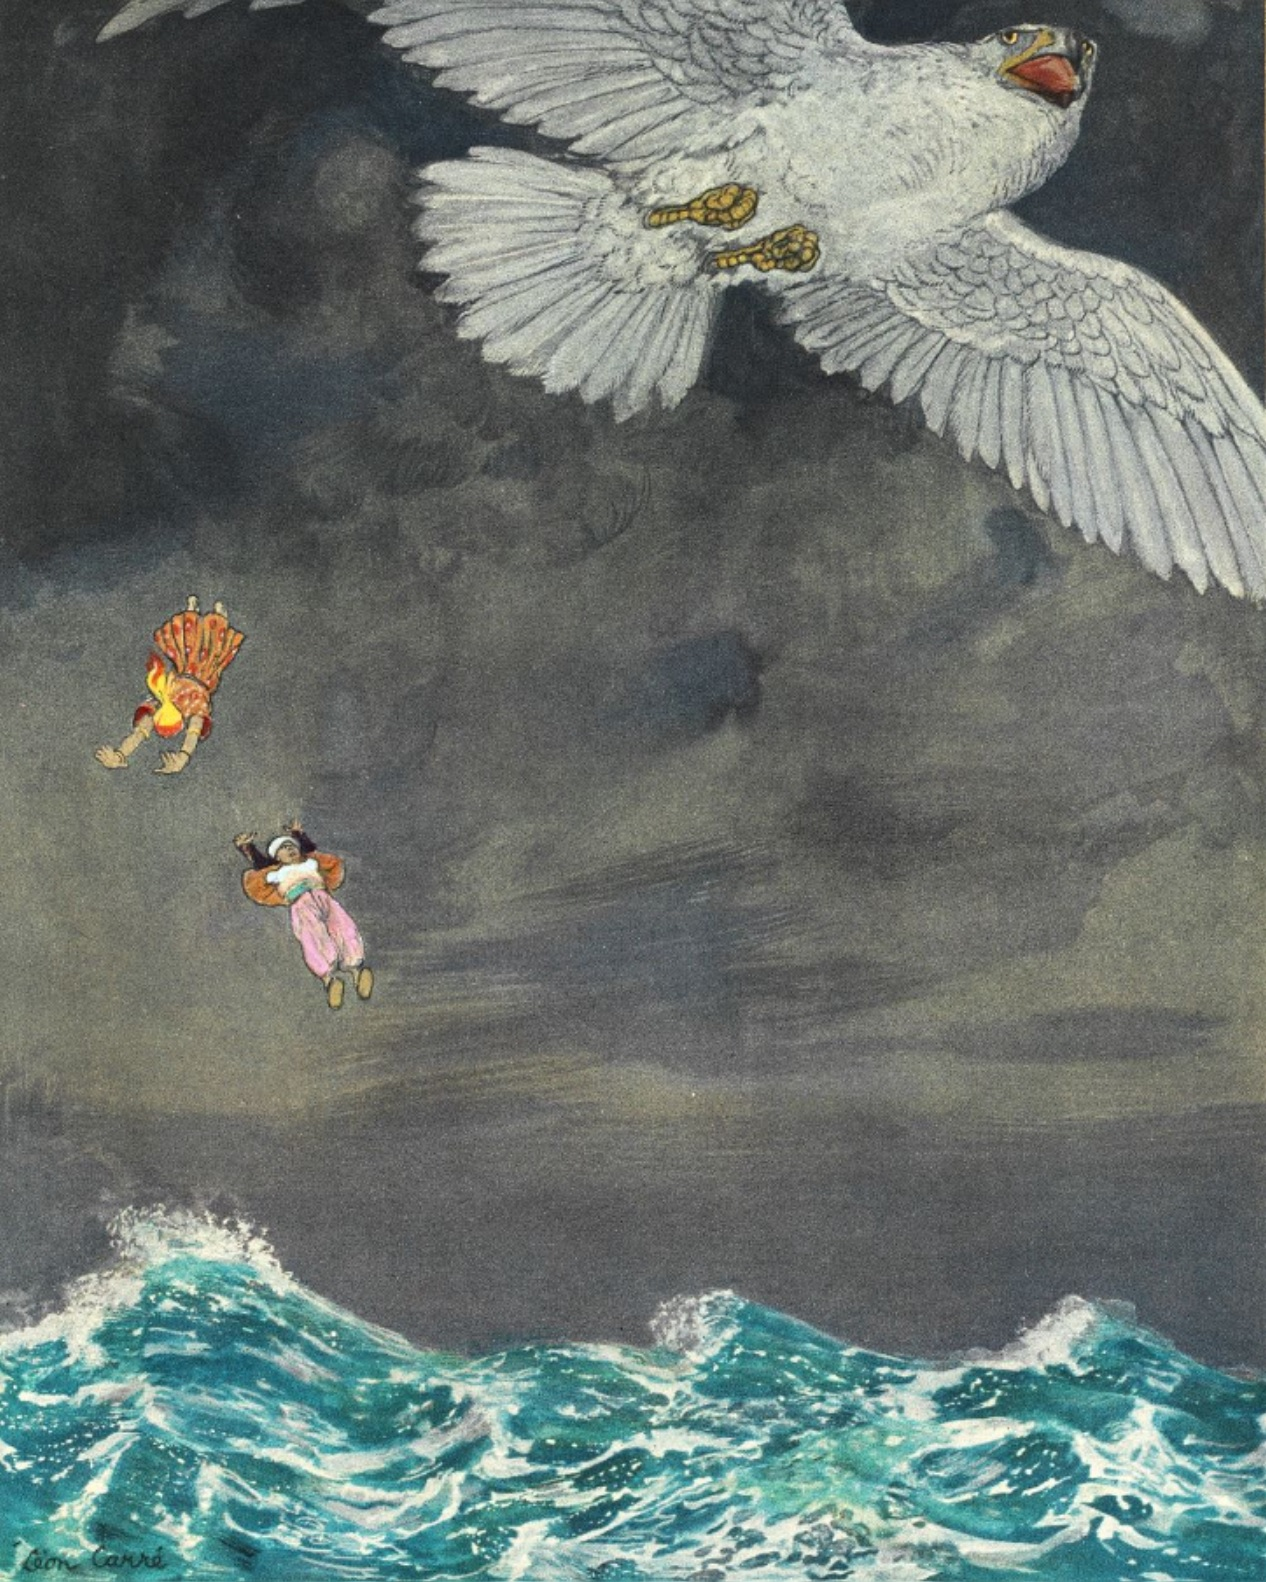
\includegraphics[height=\figsize]{illustrations/volume_7/T07, n0882 - Les séances charmantes de l'adolescence nonchalante [Le jeune garçon à la tête dure].jpg}
\end{figure}

\textit{\\
"...l’oiseau chatouillé fit un soubresaut de travers, tant la chose lui fut désagréable, et lâcha ce qu’il tenait, à savoir le frère et la sœur. Et ils tombèrent dans la mer."} \\
—T07, n0882 - Les séances charmantes de l'adolescence nonchalante [Le jeune garçon à la tête dure] \\~\\
\textit{"The sensitive bird turned a somersault in the air and instinctively loosed his grip upon the captives. The two children fell into the sea..."} \\
—V04, n0882 - Sweet tales of careless youth [Hard-head]

\newpage

\section{n0884}
\textbf{\Large{Sweet tales of careless youth [The he-goat and the king's daughter]}} \\

\begin{figure}[ht]
\centering
\includegraphics[height=\figsize]{illustrations/volume_7/T07, n0884 - Les séances charmantes de l'adolescence nonchalante [Histoire du bouc avec la fille du roi].jpg}
\end{figure}

\textit{\\
"...le bouc embrassa la terre entre les mains de son épouse, et, se secouant soudain, il rejeta sa peau de bouc et se changea en un adolescent beau comme l’ange Harout."} \\
—T07, n0884 - Les séances charmantes de l'adolescence nonchalante [Histoire du bouc avec la fille du roi] \\~\\
\textit{"...he kissed the earth between his wife's hand and with a sudden shake threw aside his skin, to appear as a youth more handsome than the angel Harut."} \\
—V04, n0884 - Sweet tales of careless youth [The he-goat and the king's daughter]

\newpage

\section{n0902}
\textbf{\Large{The tale of the magic book}} \\

\begin{figure}[ht]
\centering
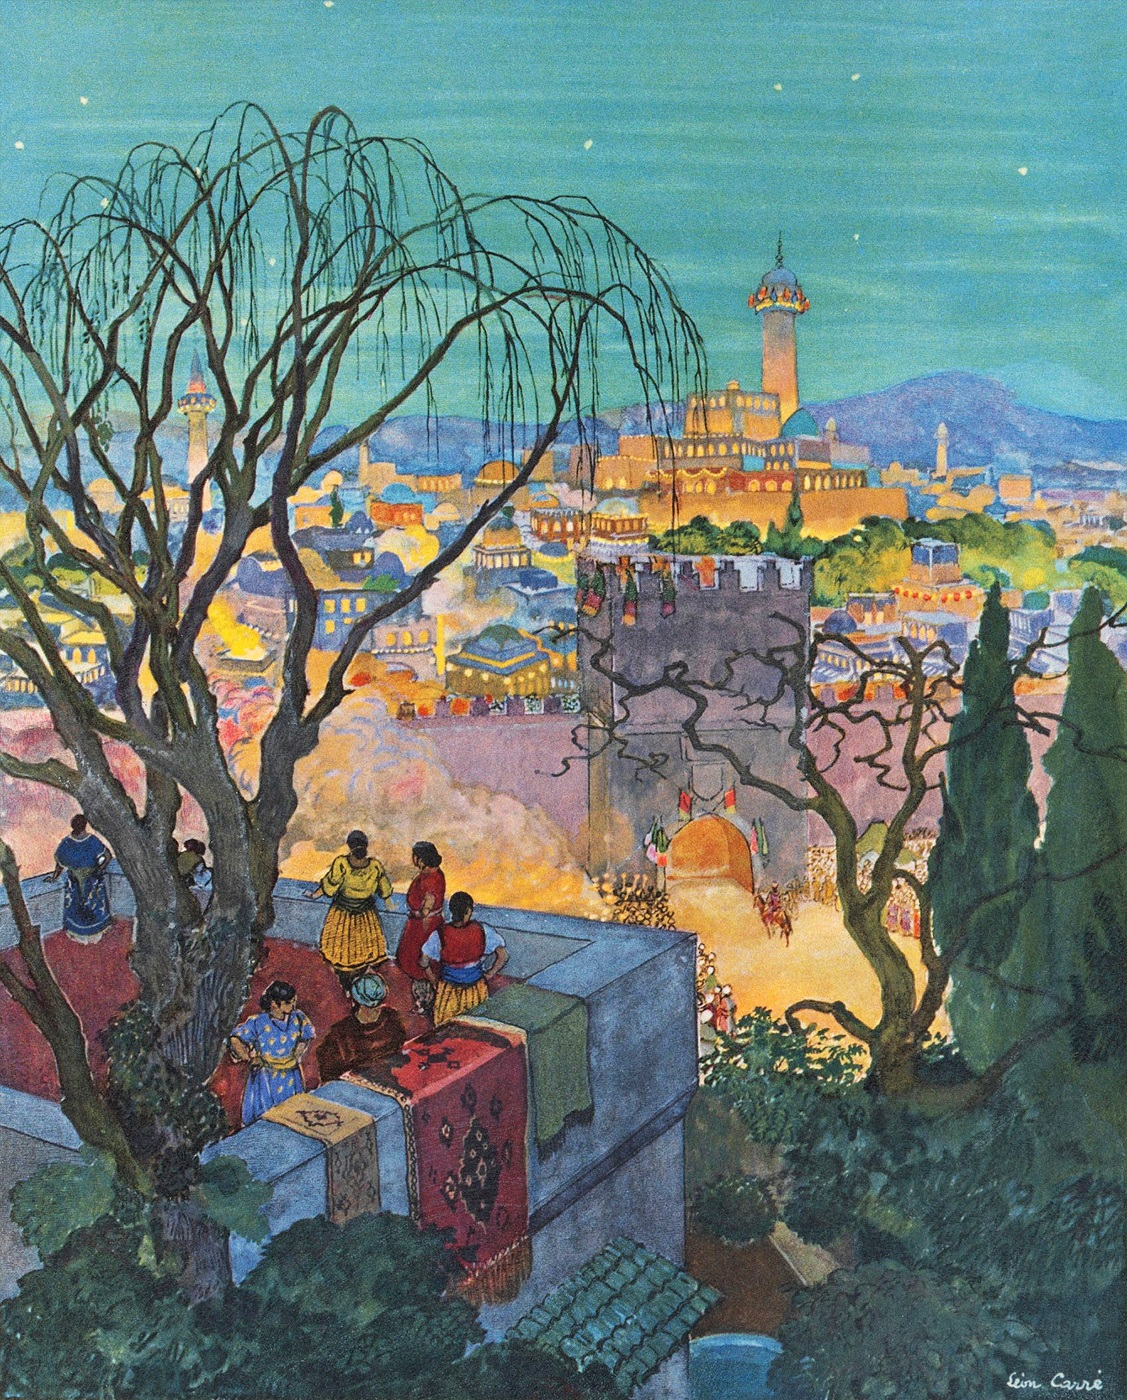
\includegraphics[height=\figsize]{illustrations/volume_7/T07, n0902 - Histoire du livre magique.jpg}
\end{figure}

\textit{\\
"...au bout de vingt jours de marche, on arriva à la ville de Koufa ; et on continua ainsi le voyage jusqu’à ce qu’on atteignît Bagdad. Et Attaf vit une cité de fortes constructions, et élégante, et riche en palais magnifiques qui montaient dans le ciel, et en délectables jardins..."} \\
—T07, n0902 - Histoire du livre magique \\~\\
\textit{"...in twenty days he reached Kufah and, not long afterwards, came in safety to the City of Peace. He found it rich in towering palaces and delectable gardens..."} \\
—V04, n0902 - The tale of the magic book

\end{document}